% !TEX program = xelatex
\documentclass[UTF8,a4paper,zihao=-4,fontset=windows]{ctexart}
\usepackage[margin=3cm]{geometry}
\usepackage{amsmath,amssymb,booktabs,array,tabularx,longtable,graphicx}
\usepackage{enumitem,caption,float,placeins,xcolor,fancyhdr,fvextra,needspace}
\usepackage{xurl}
\usepackage[hidelinks,unicode]{hyperref}
\usepackage{microtype}
\setmonofont{Consolas}
\xeCJKDeclareCharClass{CJK}{"2103}
\setlength{\parindent}{2em}
\setlength{\parskip}{0.12em}
\setlength{\emergencystretch}{3em}
\linespread{1.12}
\setlist{nosep,leftmargin=2em}
\captionsetup{font=small,labelfont=bf,labelsep=quad,skip=5pt}
\ctexset{section={format=\Large\bfseries,beforeskip=1.1ex plus .4ex,afterskip=.65ex},subsection={format=\large\bfseries,beforeskip=.85ex plus .3ex,afterskip=.5ex},subsubsection={format=\normalsize\bfseries}}
\pagestyle{fancy}
\fancyhf{}
\fancyfoot[C]{\thepage}
\renewcommand{\headrulewidth}{0pt}
\setlength{\headheight}{14pt}
\setlength{\footskip}{18pt}
\renewcommand{\arraystretch}{1.18}
\renewcommand{\topfraction}{0.95}
\renewcommand{\bottomfraction}{0.9}
\renewcommand{\textfraction}{0.05}
\renewcommand{\floatpagefraction}{0.8}
\setcounter{topnumber}{4}
\setcounter{totalnumber}{5}
\setlength{\textfloatsep}{11pt plus 2pt minus 2pt}
\setlength{\floatsep}{9pt plus 2pt minus 2pt}
\newcommand{\unit}[1]{\ensuremath{\,\mathrm{#1}}}
\newcommand{\celsius}{\ensuremath{\,{}^\circ\mathrm{C}}}
\newcommand{\Cmax}{C_{\max}}
\newcommand{\rhoe}{\rho_{\mathrm{eff}}}
\newcommand{\rhod}{\rho_{\mathrm d}}
\newcommand{\Ds}{\mathrm D_{\mathrm s}}
\newcommand{\dd}{\mathop{}\!\mathrm d}
\newcommand{\sourcecode}[2]{\Needspace{6\baselineskip}\subsection{#1}\noindent{\footnotesize\nolinkurl{#2}}\par\smallskip\VerbatimInput[fontsize=\fontsize{8}{9.5}\selectfont,breaklines=true,breakanywhere=true,numbers=left,numbersep=4pt,xleftmargin=1.6em,frame=single,framesep=3pt]{#2}\par}
\newcommand{\codegroup}[1]{\Needspace{10\baselineskip}\subsection{#1}}
\hypersetup{pdftitle={考虑变物性与径向收缩的圆柱药材干燥模型},pdfauthor={},pdfsubject={四问论文初稿},pdfkeywords={药材干燥,变物性,材料坐标,有限体积,严格阈值}}
\begin{document}
\begin{center}
{\LARGE\bfseries 考虑变物性与径向收缩的\par 圆柱药材干燥模型\par}
\vspace{0.7em}
{\large\bfseries 摘\quad 要}
\end{center}
针对圆柱药材热风干燥中的内部温度、干基含水率及终止时间，依据题给环境、分问物性与半径记录，建立有效传热传质模型。以径向模型计算中截面分布，以轴对称二维模型检验端部影响；采用守恒型有限体积与独立配点离散、隐式时间积分及未舍入极值判据，区分输出精度与模型适用范围。

第一问采用附录2的常热物性和非线性扩散系数，得到1800\unit{s}轴心、表面温度分别为33.5753\celsius、36.7856\celsius，含水率分别为2.5500、1.5102\unit{kg/kg}。

第二问从共同初态全程采用附录3，联立更新局部温度与含水率，完成逐秒全过程输出；3\unit{h}轴心、表面温度为49.8495\celsius、49.9664\celsius，含水率为1.7662、1.0081\unit{kg/kg}。

第三问以最大含水率低于0.15\unit{kg/kg}为终止要求，在4\unit{h}后维持末小时均值环境的条件下，一维执行时长为\textbf{57.4741\unit{h}}；二维直接终点节点场支持其保守方向。

第四问引入附录4和观测半径历程，在恒长度、均匀径向材料收缩假设下，用材料坐标消去移动边界并保持干基质量账本一致，得到一维条件执行时长\textbf{51.0921\unit{h}}。相较同附录4恒半径情景，规定收缩使模型时长缩短约60.65\%，该差异包含几何与所选干基边界标度的共同作用。

配对计算表明，中截面近似不能直接推广至整根总失水。4\unit{h}后温度降低1\unit{K}的受控情景使第三、四问根分别延后约1.87\unit{h}、1.64\unit{h}，远大于已检查数值差。模型尚未统一闭合真实气固平衡、组分密度与相变能量；第四问精细二维终点仍需直接补证，现有校正估计不构成连续全域严格界。所得结果用于题给系数与明确工况假设下的条件分析。

\vspace{0.7em}
\noindent\textbf{关键词：}药材干燥；变物性；材料坐标；径向收缩；阈值事件
\clearpage
\label{body:start}
\renewcommand{\thetable}{S\arabic{table}}
\renewcommand{\theHtable}{pre.\arabic{table}}
\section{问题重述与建模思路}
热风干燥通过外界换热和水分交换改变药材内部状态，外表面的变化不能直接代表轴心或整根的状态。题设对象为长25\unit{cm}、初始半径2\unit{cm}的近似圆柱药材，初始温度28\celsius、干基含水率2.55\unit{kg/kg}。环境记录、半径记录及分问物性构成给定输入\cite{problem}。本文依次处理四项任务：常热物性下的1800\unit{s}预热分布；变物性下的全过程演化及前3\unit{h}规定表；各处含水率低于0.15\unit{kg/kg}的终止要求；考虑观测收缩后的过程与时长。

四问在机制和输出要求上递进，初态并不首尾串接。问题二和三共享从初态开始的附录3轨迹；问题四另从初态使用附录4。计算采用两层空间描述：把题表的到中心距离解释为轴向中截面内的半径，以一维径向模型输出；同时计算有限长圆柱的轴对称二维场，检查中截面、端部与全域最湿位置。该解释由数值对照检验，不能作为题面已经指定中截面的事实。

圆柱有效扩散模型便于利用题给参数，并与圆环控制体离散相匹配\cite{dasilva2014}。对收缩情形，采用随材料运动的参考坐标，可以把移动表面变为固定边界。已有干燥研究使用材料输运与移动网格组织热质耦合\cite{adrover2020,wu2022}，但其他材料的平衡含水率、孔隙关系和经验收缩系数不能直接迁移。本题的具体方程由题给干基定义、选定材料运动和外法向通量重新建立。

\section{数据处理、基本假设与符号}
\subsection{数据时域与插值}
附件1含0--14400\unit{s}的环境记录，采样间隔为60\unit{s}。对记录点之间的温度和空气水分量分别线性插值，保留原采样值，不作反向参数拟合。为计算数十小时干燥过程，4\unit{h}后采用末小时61点的算术均值：
\begin{equation}
T_a=49.9989344262\celsius,\qquad b=0.04998754098\unit{kg/kg}.
\label{eq:future}
\end{equation}
其中$b$的含义见下一节。这是数据之外的环境延拓假设。使用时间加权均值、名义平台或其他后段工况会形成不同情景，不因某情景更接近通常2--3天而选择其参数。

附件2含145个半径记录，采样间隔为1800\unit{s}，覆盖0--72\unit{h}。半径由\unit{cm}换算为\unit{m}后分段线性插值；它保持记录点和单调性，避免引入未经证实的过冲。第四问主终点位于观测区间内，无须外推半径。时间积分在环境与半径的折点处分段重启，以免跨折点的光滑性假设影响误差控制。

\subsection{共同假设与有效量解释}
\begin{enumerate}
\item 药材近似轴对称连续介质，初始温度和含水率均匀；分问物性在当前位置按局部状态取值。主径向模型忽略端面，二维验证包含侧面和端面交换。
\item 材料干基含水率为$C=m_w/m_d$。附件空气量记为$y_a$，表面采用有效映射$b=g(y_a,T_s,\ldots)$；现行计算取$g(y_a,\ldots)=y_a$。它是未经材料标定的恒等映射，不能把$b$直接称为实测药材平衡含水率。
\item 换热、传质系数取$h_T=25\unit{W/(m^2K)}$、$h_m=8\times10^{-7}\unit{m/s}$。题面在附录2给出两系数，后问未另给时沿用该值；$h_m$属于材料干基驱动力标度，不自动等于气相浓度模型中的气膜系数。
\item 题给$\rho c_p$用于有效热容量，记为$\rhoe c_p$；真实干质量另由$\rhod$账本描述。不同时强制$\rho/(1+C)$为真实干密度。本模型无显式蒸发潜热、液态扩散携焓和机械功项，不能据有效热方程宣称真实能量闭合。
\item 前三问固定几何、干骨架静止；第四问取长度$L=L_0$、均匀径向材料收缩，边界按附件2给定。内部仿射运动是额外假设，单凭外半径不能唯一识别。
\end{enumerate}

\begin{table}[htbp]
\centering\small
\caption{主要符号及单位}\label{tab:symbols}
\begin{tabularx}{\linewidth}{@{}lXl@{}}
\toprule 符号&含义&单位\\\midrule
$T,T_K$&材料摄氏温度、绝对温度，$T_K=T+273.15$&$^\circ\mathrm C,\mathrm K$\\
$C,b$&材料干基含水率、有效材料边界值&$\mathrm{kg/kg}$\\
$r,z,R,L$&半径坐标、轴向坐标、当前外半径、总长度&$\mathrm m$\\
$\rhoe,\rhod$&有效容量中的密度、单位当前体积的干物质密度&$\mathrm{kg/m^3}$\\
$c_p,k,D$&比热容、导热系数、有效水分扩散系数&见表\ref{tab:properties}\\
$v_s,J$&材料速度、材料映射的体积雅可比&$\mathrm{m/s},1$\\
$\xi,x$&参考坐标$\xi=r/R$、配点坐标$x=\xi^2$&$1$\\
$t_*,t_{\mathrm{exec}}$&最大含水率等于阈值的根、正式执行时刻&$\mathrm s$\\
\bottomrule
\end{tabularx}
\end{table}

\subsection{分问物性}
表\ref{tab:properties}保留题给公式。所有指数中的温度使用$T_K$，材料水分变量均为干基$C$，不能与文献湿基量互换。
\begin{table}[htbp]
\centering\small
\caption{题给物性与本文使用方式}\label{tab:properties}
\setlength{\tabcolsep}{4pt}
\begin{tabularx}{\linewidth}{@{}lXXX@{}}
\toprule&问题一&问题二、三&问题四\\\midrule
$\rhoe\ (\mathrm{kg/m^3})$&$820$&$650+128C$&$760+90C$\\
$c_p\ (\mathrm{J/(kg\,K)})$&$2600$&$1450+\dfrac{2736C}{1+C}$&$1850+\dfrac{2150C}{1+C}$\\[5pt]
$k\ (\mathrm{W/(m\,K)})$&$0.36$&$0.21+\dfrac{0.38C}{1+C}$&$0.12+\dfrac{0.20C}{1+C}$\\[5pt]
$D\ (\mathrm{m^2/s})$&$7\times10^{-9}e^{-0.89/C}$&$\begin{gathered}2.4\times10^{-3}e^{-0.45/C}\\{}\times e^{-3850/T_K}\end{gathered}$&$\begin{gathered}4.2\times10^{-4}e^{-0.30/C}\\{}\times e^{-3850/T_K}\end{gathered}$\\
\bottomrule
\end{tabularx}
\end{table}

\section{统一传热传质模型与数值方法}
\subsection{通用方程与初边值条件}
设$\Ds/\dd t=\partial_t+v_s\cdot\nabla$为材料导数。本文有效热方程为
\begin{equation}
\rhoe(C)c_p(C)\frac{\Ds T}{\dd t}
=\nabla\cdot\bigl(k(C)\nabla T\bigr).
\label{eq:heat}
\end{equation}
由干物质和水分账本得到
\begin{equation}
\partial_t\rhod+\nabla\cdot(\rhod v_s)=0,\qquad
\rhod\frac{\Ds C}{\dd t}=\nabla\cdot\bigl(\rhod D(T,C)\nabla C\bigr).
\label{eq:moisture}
\end{equation}
在固定骨架或本文均匀径向收缩假设下，$\rhod$空间均匀，可以从水分方程约去；时间变化的体积不应再向干基变量额外添加浓缩源。外法向为$n$，表面条件为
\begin{equation}
-k\partial_nT=h_T(T_s-T_a),\qquad
-D\partial_nC=h_m(C_s-b).
\label{eq:boundary}
\end{equation}
当$C_s>b$时外向失水为正；若边界关系改变导致$C_s<b$，不能继续强制只许失水。轴线和二维中面满足零法向梯度。初态统一为
\begin{equation}
T(r,z,0)=28\celsius,\qquad C(r,z,0)=2.55\unit{kg/kg}.
\end{equation}
在一维固定圆柱中，散度取$r^{-1}\partial_r(r\,\cdot)$；轴对称二维再加$\partial_z(\cdot)$。变系数保留在散度内部，不能将$k(C)$或$D(T,C)$简单提出算子；$\rhoe c_p$乘温度变化率也不能直接改写为$\partial_t(\rhoe c_pT)$。

\subsection{守恒离散与独立配点计算}
有限体积法按圆环控制体积分方程，权重取$w_i=(r_{i+1/2}^2-r_{i-1/2}^2)/2$，轴线处内侧面积自然为零。相邻单元共用同一面通量，变系数采用与面连续性相容的插值；外表面纳入Robin通量。内部通量相消，使离散总量与边界交换具有直接对应关系。二维使用圆环与轴向控制体的乘积权重，并同时处理端面。圆柱干燥的控制体方法可参见文献\cite{dasilva2014}，本题系数和边界按表\ref{tab:properties}重新指定。

为交叉检验有限体积结果，对问题二至四另用Chebyshev配点和隐式Radau积分\cite{scipy}。令$x=(r/R)^2$，圆柱径向算子变为$4R^{-2}\partial_x(x\,\cdot)$。对可分离的$D=A(T)f(C)$，定义单调原函数
\begin{equation}
U(C)=\int_0^C f(s)\dd s,\qquad
D\nabla C=A(T)\nabla U.
\label{eq:primitive}
\end{equation}
配点在$U$上构造水分梯度，以避免直接插值较陡的$C$剖面。问题三的$f(C)=e^{-0.45/C}$，问题四为$e^{-0.30/C}$；温度因子仍按局部$T_K$更新，不能以常数代替温湿耦合。表面温度与含水率由联立Robin代数方程求解，Jacobian包含其对内部未知量的响应。

时间推进采用自适应隐式BDF或Radau方法，在输入折点分段积分，失败时停止并报告，不以截断负值掩盖求解问题。问题一正式高分辨率有限体积与独立参考相互检验；问题二、三现行统一轨迹使用80阶Radau；问题四主轨迹使用120阶配点并有160阶及独立时间方法对照。导出值与原数组的一致性、不同离散的接近程度和物理模型正确性属于不同检验，不用单一求解成功标记替代三者。

\subsection{事件、输出与可追溯性}
定义指定空间区域上的最湿值$\Cmax(t)=\max C(\cdot,t)$。等号事件和严格执行分别满足
\begin{equation}
\Cmax(t_*)=0.15,\qquad\Cmax(t_{\mathrm{exec}})<0.15.
\label{eq:event}
\end{equation}
停止判断使用未舍入值；显示为0.1500的表格数不能区分阈值两侧。对配点解，除检查节点外，还利用式\eqref{eq:primitive}的单调性查找重构多项式的全部实驻点，避免只看轴心而漏掉内部极值。连续二维严格界则需进一步控制空间、时间及重构误差，不能由节点值直接推出。

问题一和二按1\unit{s}输出，问题三和四按60\unit{s}输出；非整步的执行时刻单独追加。固定径向采样间隔为0.1\unit{cm}。第四问在当前实际半径内取值，域外为空白，当前表面另外列出。每个情景保存未舍入数组、求解配置和图表数据，论文中的规定四位表值由对应数组生成，避免从图像或已舍入中间表反算。

\FloatBarrier
\setcounter{table}{0}
\renewcommand{\thetable}{\arabic{table}}
\renewcommand{\theHtable}{body.\arabic{table}}
\section{第一问：预热阶段的径向分布}
\label{sec:q1}

\subsection{常热物性与非线性水分扩散}
第一问在前$1800\unit{s}$内使用附录2参数\cite{problem}。将共用方程
\eqref{eq:heat}--\eqref{eq:boundary}中的热容量、导热率分别取为
$820\times2600\unit{J/(m^3\cdot K)}$和$0.36\unit{W/(m\cdot K)}$，
水分扩散系数取$D(C)=7\times10^{-9}\exp(-0.89/C)\unit{m^2/s}$。
本问的$D$不依赖温度，热方程也不依赖含水率，因此两个场可分别求解，
不将其称为双向热质耦合模型。水分方程仍为非线性方程；对光滑解，
散度项除$D$乘拉普拉斯算子外还含$D'(C)C_r^2$，不能删去此项。

采用以轴心和表面为真实节点的圆环有限体积离散，每个内部界面的通量在
相邻控制体中符号相反；圆柱轴心用积分极限处理，不直接计算$1/r$。
时间推进使用隐式BDF方法\cite{scipy}，在每个环境输入折点重新启动积分并
传递末态。正式径向区间数为10240，相对容差$2\times10^{-12}$，最大步长
$3\unit{s}$。规定的$1\unit{s}$是输出间隔，不是积分固定步长。
均匀初态与初始表面Robin条件在角点不相容，计算保留题给初值，允许在
$t>0$形成早期边界层，不人为降低初始表面含水率。

\subsection{规定结果与预热规律}
表\ref{tab:q1-temperature}和表\ref{tab:q1-moisture}给出规定的七个时刻、
五个径向位置。\texttt{result1.xlsx}从第1秒至第1800秒，每隔
$0.1\unit{cm}$输出21个位置的温度和干基含水率，共75600个数值；
计算不提前舍入，输出统一显示四位小数。

\begin{table}[htbp]
\centering\small
\caption{30分钟内药材中截面温度（$^\circ$C）}
\label{tab:q1-temperature}
\input{tables/q1_temperature.tex}
\end{table}

\begin{table}[htbp]
\centering\small
\caption{30分钟内药材中截面干基含水率（kg/kg）}
\label{tab:q1-moisture}
\input{tables/q1_moisture.tex}
\end{table}

$1800\unit{s}$时轴心、表面温度分别为33.5753\celsius{}和
36.7856\celsius，均低于该时刻环境温度41.5130\celsius。表面先响应，
轴心因传导而滞后。由未舍入值计算，径向温差为$3.2102\unit{K}$。
同期表面含水率降至$1.5102\unit{kg/kg}$，轴心实际含水率约为
$2.5499924\unit{kg/kg}$，四位显示仍为2.5500；因此不能把表中轴心数字
未变解释为水分数学上严格不变。

\begin{figure}[htbp]
\centering
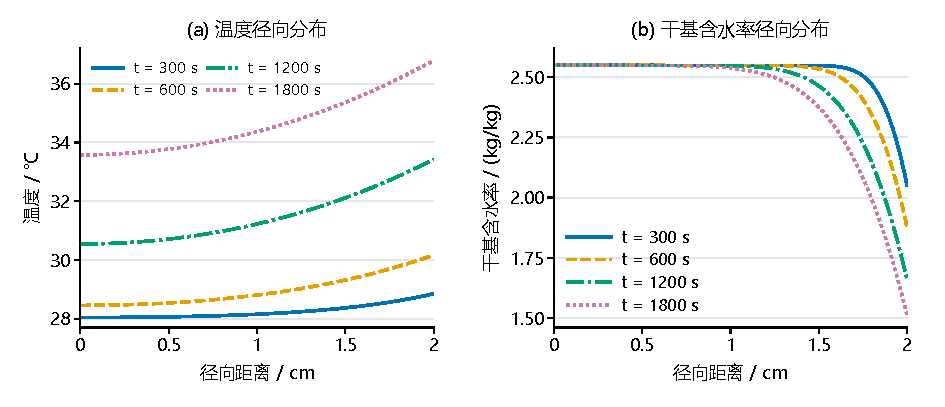
\includegraphics[width=0.94\textwidth]{figures/q1_profiles.pdf}
\caption{第一问不同时刻的径向温度与干基含水率分布。}
\label{fig:q1-profiles}
\end{figure}

图\ref{fig:q1-profiles}显示，升温已遍及所考察的径向位置，而水分变化
主要集中在表层。末时$r=1.5\unit{cm}$处的含水率为2.3755，较初值
下降约6.84\%，$r=1.0\unit{cm}$处仍为2.5383。这里不存在严格截断的
扩散前沿；描述受影响层厚度时需要先规定含水率变化阈值。

以共同尺度$R$比较扩散时间：初始热扩散率
$\alpha=k/(\rho c_p)=1.6886\times10^{-7}\unit{m^2/s}$，
$D(C_0)=4.9377\times10^{-9}\unit{m^2/s}$，故
$R^2/\alpha=2368.89\unit{s}$、$R^2/D(C_0)=81010.11\unit{s}$，
两者相差34.20倍。这解释了预热阶段热响应快于水分响应；因失水使$D$
继续减小，初始扩散时间不是最终烘干时长。
圆柱平均须按$r\,\mathrm dr$加权，得到末时中截面平均温度
35.1679\celsius、平均含水率$2.2936\unit{kg/kg}$；它们不替代最湿点，
也不能直接当作包含端部效应的整根平均量。

\subsection{数值可信范围}
温度采用贝塞尔特征函数展开作独立参考，水分采用
$x=(r/R)^2$变换的Chebyshev配点与非线性表面条件消元作独立空间参考。
正式解与参考在全部规定输出点的最大温差为
$7.29\times10^{-9}\unit{K}$，含水率差为
$1.52\times10^{-6}\unit{kg/kg}$；全部75600个正式输出四位一致。
固定正式网格收紧时间控制后，温湿差分别约
$5.03\times10^{-10}\unit{K}$和$8.15\times10^{-11}\unit{kg/kg}$。
接近舍入分界的数值必须逐项核对，不能仅凭最大误差小于半个末位单位
推断整张表四位一致。

同物理条件的$80\times128$有限圆柱二维配对，在前$1800\unit{s}$
已检查采样点的中截面最大温湿差约为
$5.65\times10^{-8}\unit{K}$与$4.09\times10^{-9}\unit{kg/kg}$，
支持本问中截面径向近似；端面局部差仍可较大，不能据此推广到整个圆柱。
以上验证支持所选有效方程的数值结果，不消除等效湿度边界、参考密度
及无显式潜热假设引入的物理不确定性。
\FloatBarrier

\FloatBarrier
\section{第二问：变物性热质耦合与全过程输出}
\label{sec:q2}

\subsection{状态反馈与全程求解}
第二问从共同初态开始，全程使用附录3物性\cite{problem}，不接续第一问
末态，也不在$1800\unit{s}$处切换公式。有效热容量
$S(C)=\rho_{\rm eff}(C)c_p(C)$和导热率随局部含水率改变，扩散率同时
依赖局部绝对温度$T_K=T+273.15$和$C$。升温改变扩散，失水又通过热容量
及导热率反馈温度，因此需联立推进两个场。

共用方程中的$k$、$D$均留在散度内。特别地，
$S^{-1}\nabla\cdot(k\nabla T)$一般不等于
$\nabla\cdot[(k/S)\nabla T]$，不能把变热扩散率直接当作热通量系数。
水分方程利用可约去的参考干密度解释；经验$\rho_{\rm eff}(C)$在这里
用于有效热容量，并不同时充当固定体积下满足真实组成守恒的湿体密度。

前$4\unit{h}$采用附件1分段线性环境，之后按统一假设保持末小时61点
算术均值：$T_a=49.9989344262\celsius$、$b=0.04998754098$。
第二问与第三问采用同一条温湿联合轨迹，积分至第三问执行端点
$206906.76\unit{s}$，即$57.4741\unit{h}$。因此第二问的完整结果
覆盖所选模型下的全过程，题设表3、表4对应的表\ref{tab:q2-temperature}、\ref{tab:q2-moisture}仅展示前$3\unit{h}$。
环境平台是超出观测范围的假设，不能将此完整时间覆盖称为数天实测验证。

全程轨迹采用80阶Chebyshev配点、原函数形式水分通量和Radau隐式
时间积分，表面温湿由Robin条件联合确定；相对容差$2\times10^{-13}$，
最大步长$30\unit{s}$，前$4\unit{h}$限制为$20\unit{s}$。
\texttt{result2.xlsx}包含两张表，每表从1秒起保存206907个时刻，即
整数秒至206906秒并追加206906.76秒；21个规定半径合计8,690,094个
温湿数值。逐秒评价联合连续解，不将不同模型的温度、水分拼接。

\subsection{规定表格及空间规律}
\begin{table}[htbp]
\centering\small
\caption{3小时内药材中截面温度（$^\circ$C）}
\label{tab:q2-temperature}
\input{tables/q2_temperature.tex}
\end{table}

\begin{table}[htbp]
\centering\small
\caption{3小时内药材中截面干基含水率（kg/kg）}
\label{tab:q2-moisture}
\input{tables/q2_moisture.tex}
\end{table}

至$3\unit{h}$，轴心、表面温度分别为49.8495\celsius、49.9664\celsius，
相差$0.1169\unit{K}$；含水率分别为1.7662、1.0081，相差
$0.7581\unit{kg/kg}$。温度接近空间均匀时，水分仍有明显梯度，
不能用均匀含水率的集中参数近似替代径向场。
按$r\,\mathrm dr$加权，平均温度为49.9043\celsius，平均含水率为
$1.3825\unit{kg/kg}$，相对初始含水率下降45.7833\%。该比例是固定参考
干密度下的有效水分减少比例，不是实测总质量损失率。

\begin{figure}[htbp]
\centering

\includegraphics[width=0.94\textwidth]{figures/q2_profiles.pdf}
\caption{第二问前3小时的中截面径向温湿分布。}
\label{fig:q2-profiles}
\end{figure}

图\ref{fig:q2-profiles}表明，初期失水集中于外层，随后内部含水率逐步
降低。第二问$0.5\unit{h}$轴心温度32.1892\celsius，低于第一问同一
时刻；这是从初态使用不同物性、尤其初始有效热容量更大的正常结果，
不是问间接口错误。第一问和第二问是不同参数情形，不能共用一段预热轨迹。

\subsection{升温促进与失水抑制的竞争}
将附录3扩散系数相对初态取对数，可精确分解为
\begin{equation}
\begin{aligned}
\ln\frac{D(t,r)}{D_0}&=H(t,r)+M(t,r),\\
H&=3850\left(\frac1{301.15}-\frac1{T_K}\right),\qquad
M=0.45\left(\frac1{2.55}-\frac1C\right).
\end{aligned}
\label{eq:q2-log-mechanism}
\end{equation}
其中$D_0=5.64168037\times10^{-9}\unit{m^2/s}$。
$H$度量沿当前轨迹的累计温度贡献，$M$度量累计含水率贡献；这是代数
分解，不能当作独立改变某一因素的因果贡献百分比。

$3\unit{h}$时，轴心与表面的$D/D_0$分别为2.1957与1.8207，说明相对
初态累计升温促进仍占优势；但最后半小时，两处扩散率分别下降约1.06\%
和3.16\%。因此“扩散系数全程单调增加”不成立。表面还曾在早期每秒
采样的第144秒达到$D/D_0=0.983282$的局部最低值。温度变化和失水抑制
的竞争随阶段变化，前3小时的累计主导关系不能直接用于判定末期干燥瓶颈。

在同一320区间有限体积网格上单独扰动交换系数，$h_m$降低、提高20\%
时，$3\unit{h}$表面含水率分别为1.1775、0.8737；相应轴心值为1.8581、
1.6921。对这一输出和扰动区间，水分交换系数的影响明显大于数值误差。
这是人为设定的确定性情景，不是参数置信区间，也不能用它替代空气量
与材料平衡含水率的基准识别\cite{dasilva2014,adrover2020}。

\subsection{独立验证与适用范围}
前3小时已有节点有限体积逐级加密至2560区间及Richardson外推，
另用独立空间离散与Radau积分核对。全程轨迹与该外推轨迹在前3小时
共同采样点的最大温差约$1.07\times10^{-9}\unit{K}$、含水率差约
$8.41\times10^{-8}\unit{kg/kg}$；前3小时温湿表及规定60个论文表值四位一致。
有限体积外推是这一前3小时交叉验证的来源，不是完整工作簿的生成方法。

长时段另与已完成的160阶BDF轨迹在全部60秒采样点及同一执行端点比较，
最大温湿差约$3.27\times10^{-9}\unit{K}$与$9.33\times10^{-9}\unit{kg/kg}$，
四位输出一致。当前869万余格工作簿与同源未舍入轨迹的舍入核对全部通过，
该检查支持导出一致性；高阶独立参考覆盖的是所列采样点，不能把导出
一致性误写成全部逐秒状态均另作了独立求解。

原有限体积有效水分账本的最大残差约$6.51\times10^{-12}\unit{kg/kg}$。
热账本核对的是有效热容量积分与边界热流，即比较
$\int\!\int S(C)T_t\,\mathrm dV\mathrm dt$与累计边界热量，
相对残差约$3.11\times10^{-11}$，并非$\int ST\,\mathrm dV$的末初差，
更不构成潜热、携焓及真实总能量已经闭合的证明。
同物理$80\times256$二维配对在前3小时已检查采样点的中截面最大温湿差
约为$1.692\times10^{-3}\unit{K}$、$2.247\times10^{-5}\unit{kg/kg}$。
这支持中截面的工程近似，但不能保证降维后所有四位显示相同；长期全域
达标须结合第三问终点证据，不能直接沿用前3小时的几何误差。
\FloatBarrier

\FloatBarrier
\input{sections/q3}
\FloatBarrier
\input{sections/q4}
\FloatBarrier
\section{降维检验与环境敏感性}
\subsection{中截面、端部与整根积分}
中截面配对需要保持相同物性、环境与边界，才能识别额外轴向交换的影响。问题一80$\times$128二维对照在0--1800\unit{s}中截面采样的最大温度差约为$5.65\times10^{-8}\unit K$，含水率差约为$4.09\times10^{-9}\unit{kg/kg}$。问题二采用最终80$\times$256对照，在前10800\unit{s}的对应差为$1.69165\times10^{-3}\unit K$与$2.24706\times10^{-5}\unit{kg/kg}$，支持中截面工程近似，但不能宣称所有四位单元均一致。

另一方面，端面交换会改变整根失水。按二维控制体权重与一维圆环权重积分得到表\ref{tab:wholebody}。表中“失水增加”定义为$(C_0-\overline C_{2D})/(C_0-\overline C_{1D})-1$，不是平均含水率的相对误差。在空间均匀干密度的共同假设下，体积权重平均等于干质量权重平均。
\begin{table}[htbp]
\centering\small
\caption{同网格保存场的整根失水对照}\label{tab:wholebody}
\begin{tabular}{@{}lrrrr@{}}
\toprule 情形与时刻&二维网格&$\overline C_{2D}$&$\overline C_{1D}$&失水增加/\%\\\midrule
问题一，1800\unit{s}&80$\times$128&2.274929&2.293532&7.2533\\
问题二，3\unit{h}&80$\times$256&1.327482&1.382492&4.7118\\
问题四，6\unit{h}&80$\times$128&1.024545&1.065198&2.7379\\
\bottomrule
\end{tabular}
\end{table}
\FloatBarrier
中截面差小与整根总量差可见并不矛盾。若用于全长平均、总失水或端部状态，应采用二维积分或明确忽略端面的近似，不能把中截面表格的精度扩展到全部工程指标。

打开端面后，配对算例显示最湿点更早达到阈值，但这尚不是一般比较定理。温度场与含水率相互耦合；即使$D$随温度增加，两个解之间的变系数通量散度也未必具有统一符号。因此问题三、四的一维执行值、二维节点场、配对校正与连续严格界分别报告。

\subsection{后段环境的受控情景}
由于式\eqref{eq:future}仅为4\unit{h}后的延拓，保持短时实测过程不变，从保存的4\unit{h}内部温湿场开展后段联立续算。每问设置原平台、温度$\pm1\unit K$和有效边界$b\pm0.005$五种情景；第四问始终使用同一观测$R(t)$。扰动幅度为人为选择的压力测试，没有作为测量不确定度或置信区间。表\ref{tab:environment}给出40阶配点的等号事件根，差值相对于同阶基线。
\begin{table}[htbp]
\centering\small
\caption{4\unit{h}后环境改变的条件根与时长差}\label{tab:environment}
\begin{tabular}{@{}lrrrr@{}}
\toprule 情景&问题三根/h&变化/h&问题四根/h&变化/h\\\midrule
原均值平台&57.473996&0&51.092003&0\\
$T_a-1\unit K$&59.341275&$+1.867279$&52.729346&$+1.637343$\\
$T_a+1\unit K$&55.688357&$-1.785639$&49.525343&$-1.566660$\\
$b-0.005$&57.382748&$-0.091249$&50.993818&$-0.098185$\\
$b+0.005$&57.584113&$+0.110117$&51.218753&$+0.126750$\\
\bottomrule
\end{tabular}
\end{table}
\begin{figure}[htbp]
\centering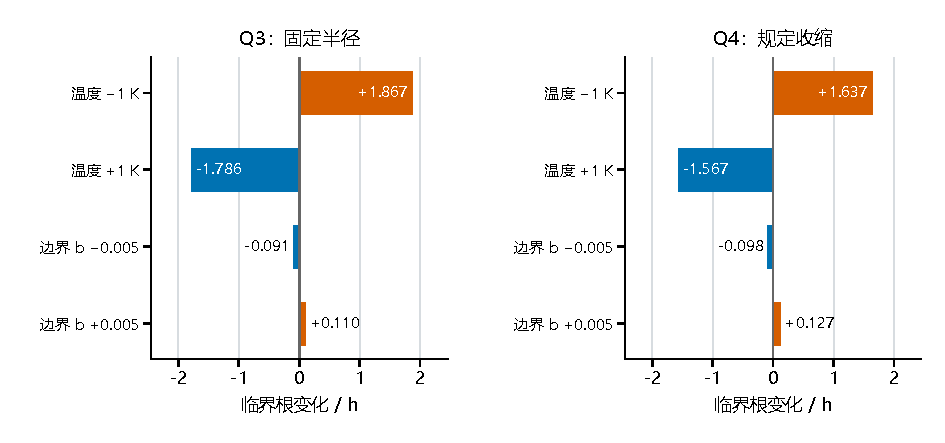
\includegraphics[width=.93\linewidth]{figures/environment_sensitivity.pdf}
\caption{后段环境情景相对同阶基线的根变化；幅度为人工设定，第四问规定半径保持不变。}\label{fig:environment}
\end{figure}
\FloatBarrier

对基线和降1\unit K情景进一步加密：问题三40阶到80阶、问题四40阶到60阶，单个根的最大变化分别约0.002951\unit{s}与0.000174\unit{s}，降温净效应的变化更小。因此小时级差不是此次降阶造成的；其他扰动没有逐一加密，表中六位小数仅便于追踪数值，不代表真实预测精度。

长期降温在既定模型内减小扩散温度因子，推迟阈值；提高$b$减小失水驱动力，也使根后移。由于两类扰动尺度不同，不能据图\ref{fig:environment}断定温度比所有湿度误差都重要。已有时间加权均值对照使问题三根变化约20.04\unit{s}，问题四改用PCHIP半径插值使根提前约12.61\unit{s}，二者也超过亚秒级一维经验数值预算。工程执行余量应建立在可用工况范围上，不能只依据四位小时的取整步长。

\section{模型适用范围与改进方向}
\subsection{气固边界与目标可达性}
材料$C$和空气$y_a$虽然都可写作\unit{kg/kg}，分母却未必相同。湿空气湿度比、相对湿度和体积蒸气浓度需分别定义\cite{ashrae}。真实气膜候选边界可写为
\begin{equation}
j_s=k_g\{c_{v,s}(C_s,T_s)-c_{v,a}\},
\label{eq:physical-interface}
\end{equation}
其中$c_{v,s}$需材料水活度或解吸关系。若将浓度差局部线性化为$c_{v,s}-c_{v,a}\approx K(C_s-b)$，才能建立$\rhod h_m=k_gK$的对应，而非直接交换系数数值。圆柱有效干燥模型与移动边界模型分别使用平衡干基含水率或气相/解吸关系\cite{dasilva2014,adrover2020}，它们没有提供本药材的标定值。

首先需要核实目标环境下的材料平衡含水率$C_{\mathrm{eq}}$是否低于0.15。若恒定环境对应$C_{\mathrm{eq}}\ge0.15$，从较高含水率开始的扩散干燥可能无法实现全域严格阈值；提高网格精度不能消除这一不可达性。缺少数据时可报告边界情景，但不能给未经标定的$C_{\mathrm{eq}}$冠以实测含义。

\subsection{经验密度与材料质量的相容性}
若同时把题给$\rho=a+b_\rho C$解释为真实当前湿体密度，则干基定义要求
\begin{equation}
\rhod(C)=\frac{a+b_\rho C}{1+C},\qquad
\frac{\dd\rhod}{\dd C}=\frac{b_\rho-a}{(1+C)^2}.
\end{equation}
前三问固定骨架的干密度应保持不变，而该经验关系随失水改变；第四问仿射材料收缩要求$\rhod$空间均匀，但非均匀$C$会给出非均匀经验干密度。本文将题给$\rho$仅用于有效容量，是对上述不相容关系的建模处置，不能说题面已经规定了这一有效化解释。

以第四问保存场作反证性积分，若强制采用真实湿密度解释，则7\unit{h}和末态的隐含干质量相对初值分别为0.71952、0.89029。保持现有$C,R$场不变，只靠改变长度凑足总干质量，需由25\unit{cm}增至34.7454\unit{cm}与28.0807\unit{cm}。这说明增加轴向收缩不能修复当前缺口；即使伸长凑平总量，局部相容性仍待解决。该诊断不等于本文独立干质量账本发生了数值泄漏，也不是新的可行伸长模型。

\subsection{相变能量与可报告的指标}
式\eqref{eq:heat}只描述有效温升，不含显式潜热。有限的$\rhoe c_p$不能在近等温而持续失水时自动补充汽化功率。为考察量级，在“初始湿密度确定干质量、全部等效失水均蒸发”的附加条件下，取诊断常数$\lambda=2.45\unit{MJ/kg}$\cite{fao}，问题一1800\unit{s}的潜热需求约45.59\unit{kJ}，原温度轨迹对流输入约4.801\unit{kJ}，比例约9.50。

问题四12\unit{h}表面温度几乎等于环境，原轨迹净对流输入接近零，而条件潜热通量$\lambda\rhod h_m(C_s-b)$约164.10\unit{W/m^2}。这一反例足以排除“题给有限$c_p$已自动包含潜热”的解释，但不是实际耗能测量。若重新联立相变，表面降温会增加热输入并改变扩散，不能拿原热输入固定不变直接倍乘干燥时间。

因此本文可报告题给有效模型的温湿分布、阈值事件和条件时长差，不能从中推出实际节能率或真实执行保证。进一步闭合应让同一真实$j_s$进入质量与能量边界，并采用一致焓基准；域内含水率下降包含水分扩散，不能全部视为局部蒸发，再重复加入体积潜热项。

\subsection{优先补强的计算与数据}
数值层面，最直接的补强是第四问正式时刻的精细二维场，配合径向加密、时间紧化及起点前史误差检查，使正阈值裕量覆盖相称误差。仅把粗网格晚期场插值到细网格，不能消除共同继承偏差；普通收敛检验也不同于连续数学误差界。

模型层面，优先比较“固定干基$h_m$”与“固定$\rhod h_m$”的条件响应，再用实测后段环境建立适用工况。若有独立失重和表面温度数据，先在短时窗核查气固关系、干质量与相变能量，验证后再延长全过程。仅有$R(t)$是边界输入，不能据其吻合宣称温湿预测或其他工况的收缩反馈已获实验验证。附录3/4与固定/收缩几何的第四格对照、非均匀材料运动可作为进一步研究，不应抢先于这些关键接口。

\FloatBarrier
\section{结论}
本文在统一有效传热传质框架下完成四问的模型、规定表格与全过程输出。问题一描述热响应领先于水分扩散的短时非均匀过程；问题二通过局部变物性联立演化，把前3\unit{h}规定表扩展至完整干燥历程；问题三将等号事件与严格执行时刻分开；问题四在给定半径历程下，用材料运动和干基守恒解释参考域方程及收缩对照。

在本文工况与模型假设下，第三、四问的一维条件执行时长分别为57.4741\unit{h}和51.0921\unit{h}。二维证据支持中截面降维，并要求对整根失水和全域终点另作检查；特别是第四问精细二维直接终点与误差裕量尚未补齐，不能据现有估计宣称连续有限圆柱严格保证。后段环境情景显示，实际工况稳定性对执行时间的影响值得优先检验。

后续改进应先明确空气与材料水分的对应关系、核查终点平衡可达性，继而在相容质量基准上联立同一界面水通量与能量。现有规定半径只能支撑条件响应，不能单独识别另一工况下的收缩反馈。上述数据需求比无依据增加模型复杂度更直接地关系到真实过程预测。

\Needspace{9\baselineskip}
\section*{AI工具使用声明}
\label{ai:declaration}
本参赛队在竞赛过程中使用了AI工具，主要用于模型方案整理与质疑、代码辅助与结果核查、文献检索辅助、图表生成以及论文初稿撰写和排版，详细使用情况见支撑材料。

本稿为AI辅助形成的初版。现有计算核对和交叉审阅由程序及代理完成，不等同于参赛队员逐项人工审核；尚未取得覆盖本版全部内容的人工修改与核验记录。正式采用前应完成并如实补充该项记录。
\input{sections/references}
\FloatBarrier
\ifdefined\BodyOnly
\else
\clearpage
\appendix
\label{appendix:start}
\section{支撑材料与完整采用代码}
\label{sec:complete-code}
支撑目录按原项目相对路径组织于\texttt{support/project/}，保存本文采用的求解、验证和后处理源码；数值输入工作簿随包提供，较大的未舍入数组和正式工作簿作为独立支撑文件保存。代码附录位于正文之后，不计入正文页数。

本稿制作阶段只进行只读材料核对、必要的后处理以及语法和入口冒烟检查，没有重新执行四问全部偏微分方程求解及工作簿导出。复现时应先核对输入与依赖，再按问题顺序在新输出目录运行；任何新的数值或模型变化均须重新验证，不能以本次文稿构建代替数值验收。

对外源码使用匿名相对路径。原历史源码保持不变；副本中的来源标记和本机专用路径只作匿名化或参数化处理，未改变物性、边界、离散通量及阈值判据。完整文件索引与运行限制见\texttt{support/README.md}。

\codegroup{运行顺序与代码范围}
首先运行\texttt{python support/launch.py smoke}，该入口只解析语法、核查副本哈希并执行白名单程序的\texttt{--help}，不会积分。完整复现须使用新的工作目录：先以附件1重建第一问和第二、三问轨迹，再用第三问专用轨迹导出表5；第四问读取附件2，完成主解、谱节点和时间算法对照、有限体积与二维对照后才能执行终点预算和工作簿导出。参数情景在各自同网格基线上比较；二维校正和直接离散场判定仍须分别报告。

第二问机制诊断依赖已验收未舍入轨迹及320单元有限体积参数情景。本文表3、表4及全程\texttt{result2.xlsx}采用后续统一轨迹；机制诊断的旧前三小时数组不替代该正式工作簿。环境敏感性程序从同一个4小时完整状态继续积分；本次编稿不重新生成这些状态。

体积较大的\texttt{NPZ}数组和正式工作簿未重复放入代码快照；复现说明列出必需外部证据及其相对路径。部分历史后处理程序没有输出参数且会在镜像目录写文件，必须在工作副本中运行；没有\texttt{--help}保护的脚本只检查语法。工作簿批量导出另需\texttt{@oai/artifact-tool}及对应Node运行时；本次没有执行此导出链。

匿名化改变了少量源码文件的字节，故使用旧冻结环境证据时，源码哈希核验可能按设计拒绝该匿名副本。这不是数值不一致证明，也不能通过关闭断言略过；应在内部原字节快照核验，或用匿名源码重新计算并建立新的源哈希记录。源码和副本的SHA256映射存于支撑清单，数值核保持不变。

\sourcecode{匿名快照启动与冒烟检查}{support/launch.py}

\codegroup{第一问求解及交付}
\sourcecode{run\_all}{support/project/q1_complete_delivery/q1_delivery/run_all.py}

\sourcecode{q1\_solver}{support/project/q1_complete_delivery/q1_delivery/source/q1_solver.py}

\sourcecode{q1\_validate}{support/project/q1_complete_delivery/q1_delivery/source/q1_validate.py}

\sourcecode{q1\_refine}{support/project/q1_complete_delivery/q1_delivery/source/q1_refine.py}

\sourcecode{q1\_rounding\_audit}{support/project/q1_complete_delivery/q1_delivery/source/q1_rounding_audit.py}

\sourcecode{q1\_excel}{support/project/q1_complete_delivery/q1_delivery/source/q1_excel.py}

\sourcecode{q1\_report}{support/project/q1_complete_delivery/q1_delivery/source/q1_report.py}

\codegroup{第二问机制与参数情景}
\sourcecode{q2\_core}{support/project/q2_refinement_delivery/runtime/source/q2_core.py}

\sourcecode{q2\_spectral}{support/project/q2_refinement_delivery/runtime/source/q2_spectral.py}

\sourcecode{q2\_tests}{support/project/q2_refinement_delivery/runtime/source/q2_tests.py}

\sourcecode{q2\_core\_original}{support/project/q2_refinement_delivery/reused/q2_core_original.py}

\sourcecode{prepare\_reused}{support/project/q2_refinement_delivery/source/prepare_reused.py}

\sourcecode{q2\_mechanism}{support/project/q2_refinement_delivery/source/q2_mechanism.py}

\codegroup{第二三问全程统一轨迹}
\sourcecode{q3\_solver}{support/project/q4_complete_delivery/v1/q123_closeout/source/legacy_q3/q3_solver.py}

\sourcecode{q3\_reference}{support/project/q4_complete_delivery/v1/q123_closeout/source/legacy_q3/q3_reference.py}

\sourcecode{solve\_unified\_q23}{support/project/q4_complete_delivery/v1/q123_closeout/source/solve_unified_q23.py}

\sourcecode{audit\_unified\_q23}{support/project/q4_complete_delivery/v1/q123_closeout/source/audit_unified_q23.py}

\codegroup{第三问现行执行点与核验}
\sourcecode{q3\_solver}{support/project/q3_refinement_delivery/source/q3_solver.py}

\sourcecode{q3\_reference}{support/project/q3_refinement_delivery/source/q3_reference.py}

\sourcecode{q3\_refined\_reference}{support/project/q3_refinement_delivery/source/q3_refined_reference.py}

\sourcecode{future\_scenarios\_from\_checkpoint}{support/project/q3_refinement_delivery/source/future_scenarios_from_checkpoint.py}

\sourcecode{export\_workbook}{support/project/q3_refinement_delivery/source/export_workbook.py}

\sourcecode{validate\_xlsx}{support/project/q3_refinement_delivery/source/validate_xlsx.py}

\sourcecode{verify\_frozen}{support/project/q3_refinement_delivery/source/verify_frozen.py}

\codegroup{第四问及有限圆柱验证}
\sourcecode{q4\_common}{support/project/q4_complete_delivery/v1/source/q4_common.py}

\sourcecode{q4\_spectral}{support/project/q4_complete_delivery/v1/source/q4_spectral.py}

\sourcecode{run\_q4}{support/project/q4_complete_delivery/v1/source/run_q4.py}

\sourcecode{check\_numerics}{support/project/q4_complete_delivery/v1/source/check_numerics.py}

\sourcecode{finalize\_q4}{support/project/q4_complete_delivery/v1/source/finalize_q4.py}

\sourcecode{package\_workbooks}{support/project/q4_complete_delivery/v1/source/package_workbooks.py}

\sourcecode{export\_workbooks}{support/project/q4_complete_delivery/v1/source/export_workbooks.mjs}

\sourcecode{geometry\_solver\_executed}{support/project/q4_complete_delivery/v1/source/geometry_solver_executed.py}

\sourcecode{geometry\_solver}{support/project/q4_complete_delivery/v1/source/geometry_solver.py}

\sourcecode{geometry\_checks}{support/project/q4_complete_delivery/v1/source/geometry_checks.py}

\sourcecode{geometry\_analysis}{support/project/q4_complete_delivery/v1/source/geometry_analysis.py}

\sourcecode{geometry\_report}{support/project/q4_complete_delivery/v1/source/geometry_report.py}

\codegroup{本次整体复审}
\sourcecode{diagnose\_saved\_fields}{support/project/q1234_overall_review_delivery/v1/reviews/physics/diagnose_saved_fields.py}

\sourcecode{environment\_probe}{support/project/q1234_overall_review_delivery/v1/source/environment_probe.py}

\sourcecode{audit\_environment\_evidence}{support/project/q1234_overall_review_delivery/v1/reviews/environment_check/audit_environment_evidence.py}

\sourcecode{audit\_saved\_geometry\_scope}{support/project/q1234_overall_review_delivery/v1/reviews/geometry/audit_saved_geometry_scope.py}

\sourcecode{audit\_geometry\_endpoints}{support/project/q1234_overall_review_delivery/v1/reviews/geometry/audit_geometry_endpoints.py}

\codegroup{本稿图表后处理}
\sourcecode{build\_assets}{support/project/paper/q1234_draft_v1/build_assets.py}


\fi
\label{document:end}
\end{document}
